\documentclass{report}
\usepackage{tikz}
    \usetikzlibrary{shapes, arrows, chains, positioning, snakes}


\begin{document}

\section{List item}
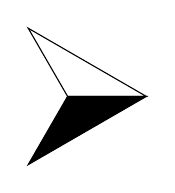
\begin{tikzpicture}
    \draw (0, 0) -- +(1, 0) -- +(120:1) -- cycle;
    \draw[fill=black] (0, 0) -- +(1, 0) -- +(-120:1) -- cycle;
\end{tikzpicture}

\begin{tikzpicture}[rotate=45]
    \draw[fill=black] (0, 0) rectangle +(1, 1);
    \draw[white, line width=2.5pt] (0, 0.5) -- +(1, 0);
    \draw[white, line width=2.5pt] (0.5, 0) -- +(0, 1);
\end{tikzpicture}
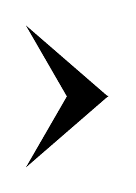
\begin{tikzpicture}
    \draw[fill=black] (0, 0) -- +(0.5, 0) -- +(120:1) -- cycle;
    \draw[fill=black, yscale=-1] (0, 0) -- +(0.5, 0) -- +(120:1) -- cycle;
\end{tikzpicture}

\begin{tikzpicture}
    \draw[fill=black] (0, 0) -- ++(0.7, 0) -- ++(120:1) -- +(-0.7, 0) -- cycle;
    \draw[fill=black, yscale=-1] (0, 0) -- ++(0.7, 0) -- ++(120:1) -- +(-0.7, 0) -- cycle;
\end{tikzpicture}
    
\end{document}
